\documentclass{beamer}
\usepackage{ctex}
\usepackage{makecell}
\usepackage{amsmath}
\usepackage{array}
\usepackage{graphicx}
\usepackage{pdfpages}
\usepackage{float}
\usepackage{fancyhdr}
\usepackage{multirow}
\usepackage{diagbox}
\usepackage{siunitx}
\usepackage{verbatim}
\usepackage{indentfirst}
\usepackage{caption}
\usepackage{circuitikz}
\usepackage{subfigure}
\usepackage{tikz}
\usepackage{pgfkeys}
\usepackage{pgffor}
\usepackage{pgfcalendar}
\usepackage{pgfpages}
\usepackage{booktabs}
\usetikzlibrary{calc,angles,positioning,intersections,arrows.meta}
\setlength{\parindent}{2em}
\title{My Recent Work}
\author{Qian Sitian}
\date{2018/7/25}
\begin{document}
\maketitle
\begin{frame}
    \titlepage
\end{frame}
\begin{frame}
    \frametitle{Outline}
    \tableofcontents
\end{frame}
\begin{frame}   
    \section{Parameter Fitting}
    \frametitle{Parameter Fitting}
    \begin{itemize}
        \item Preview
        \item Parameters to Obserables
        \item Obserables to Parameters
    \end{itemize}
\end{frame}
\begin{frame}
    \frametitle{Preview}
    \subsection{Preview}
    Basic Information:
    \begin{itemize}
        \item Model:\\Collective 
        ow in 2.76 A TeV and 5.02 A TeV Pb+Pb
        collisions
        \\
        Arxiv:1703.10792
        \item Motivation:\\Applying Bayesian parameter estimation to relativistic heavy-ion collisions:
        simultaneous characterization of the initial state and quark-gluon plasma medium
        \\
        Arxiv:1605.03954
    \end{itemize}
\end{frame}
\begin{frame}
    \frametitle{Target}
    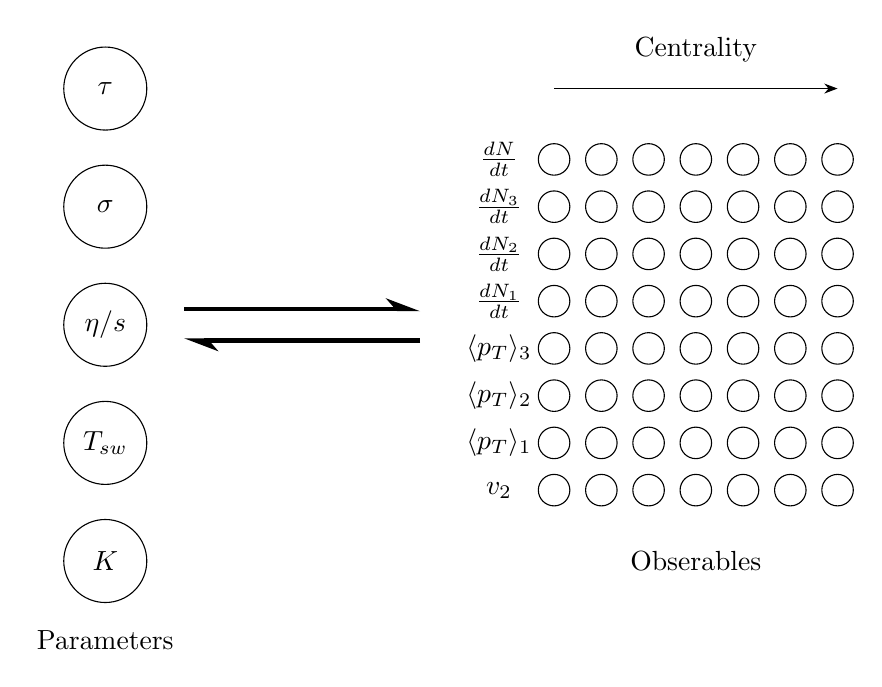
\begin{tikzpicture}
        \node[circle,draw] at (0,3+4)[minimum size=30pt] {$\tau$};
        \node [circle,draw]at (0,1.5+4)[minimum size=30pt] {$\sigma$};
        \node [circle,draw]at (0,0+4)[minimum size=30pt] {$\eta/s$};
        \node [circle,draw]at (0,-1.5+4)[minimum size=30pt] {$T_{sw}$};
        \node [circle,draw]at (0,-3+4)[minimum size=30pt] {$K$};
        \node at(0,-4+4){Parameters};
        \draw [arrows = {-Stealth[harpoon]},ultra thick] (1,4.2) -- (4,4.2);
        \draw [arrows = {-Stealth[harpoon]},ultra thick] (4,3.8) -- (1,3.8);
        \foreach \x in{0,1,2,3,4,5,6,7} \foreach \y in {0,1,2,3,4,5,6}
            \draw  (7.5+0.6*\y-1.8,4+0.6*\x-2.1) circle(0.2cm);
        \foreach \name/\x in{v_2/0,\langle p_T\rangle_1/1,\langle p_T\rangle_2/2,\langle p_T\rangle_3/3,\frac{dN_1}{dt}/4,\frac{dN_2}{dt}/5,\frac{dN_3}{dt}/6,\frac{dN}{dt}/7}
            \node at (5,4+0.6*\x-2.1) {$\name$};
        \node at(7.5,-3+4){Obserables};
        \node at(7.5,3.5+4){Centrality};
        \draw [{arrows = {-Stealth[reversed, reversed]}},] (7.5-1.8,7) -- (7.5+1.8,7);
    \end{tikzpicture}
\end{frame}
\begin{frame}
    \frametitle{Data}
    \begin{itemize}
        \item Initial:
 
        \begin{table}
            \centering
            \begin{tabular}{c|c|c|c|c}
                \toprule
                $\tau$&$\sigma$&$\eta/s$&$T_{sw}$&$K$\\
                \midrule
                0.2&0.2&0.02&0.15&0.4\\
                0.6&0.6&0.08&0.24&0.8\\
                0.9&1.0&0.12&0.4&1.2\\
                \bottomrule
            \end{tabular}
        \end{table}
    \item Divide:

    $$ Total:3^5=243\Rightarrow\left\{
\begin{aligned}
Train:& 220 \\
Test:& 23
\end{aligned}
\right.
$$
    \end{itemize}
    
\end{frame}
\begin{frame}
    \subsection{Parameters to Obserables}
    \frametitle{Parameters to Obserables}
    \begin{itemize}
        \item Network
        \item Result
    \end{itemize}
\end{frame}
\begin{frame}
    \frametitle{Network}
    %tikz画图
\end{frame}
\begin{frame}
    \frametitle{Result}
\end{frame}

\end{document}